\Chapter{Megvalósítás}


\Section{A rendszer felépítése}

% Ide egy magasabb szintű architekturális áttekintés kerül.


A webalkalmazás fejlesztése során fontos szempont volt az alapvető technológiai döntések meghozatala. Az alkalmazásom három fő komponensre épül: adatbázis, backend és frontend. Az adatbázis rétegként MySQL-t\cite{MySQL} használok, mely hatékonyan tárolja és kezeli az adatokat. A backendet Java Spring Boot\cite{spring_boot} keretrendszer segítségével építem fel, ami biztosítja az üzleti logika végrehajtását és az adatok kezelését. A frontend felelős a felhasználói felület megjelenítéséért és kezeléséért. Ehhez az Angular\cite{angular} keretrendszert alkalmazom, ami modern és komponensalapú megközelítést biztosít.\\
\\
Ezek a technológiák összehangoltan működnek, hogy egy erőteljes, hatékony és felhasználóbarát webalkalmazást hozzanak létre. A MySQL\cite{MySQL} adatbázis, a Java Spring Boot\cite{spring_boot} backend és az Angular\cite{angular} frontend kombinációja lehetővé teszi számomra, hogy magas színvonalú alkalmazást fejlesszek ki. Ez megfelel a felhasználók elvárásainak és az iparági követelményeknek.

\begin{figure}[h]
\centering
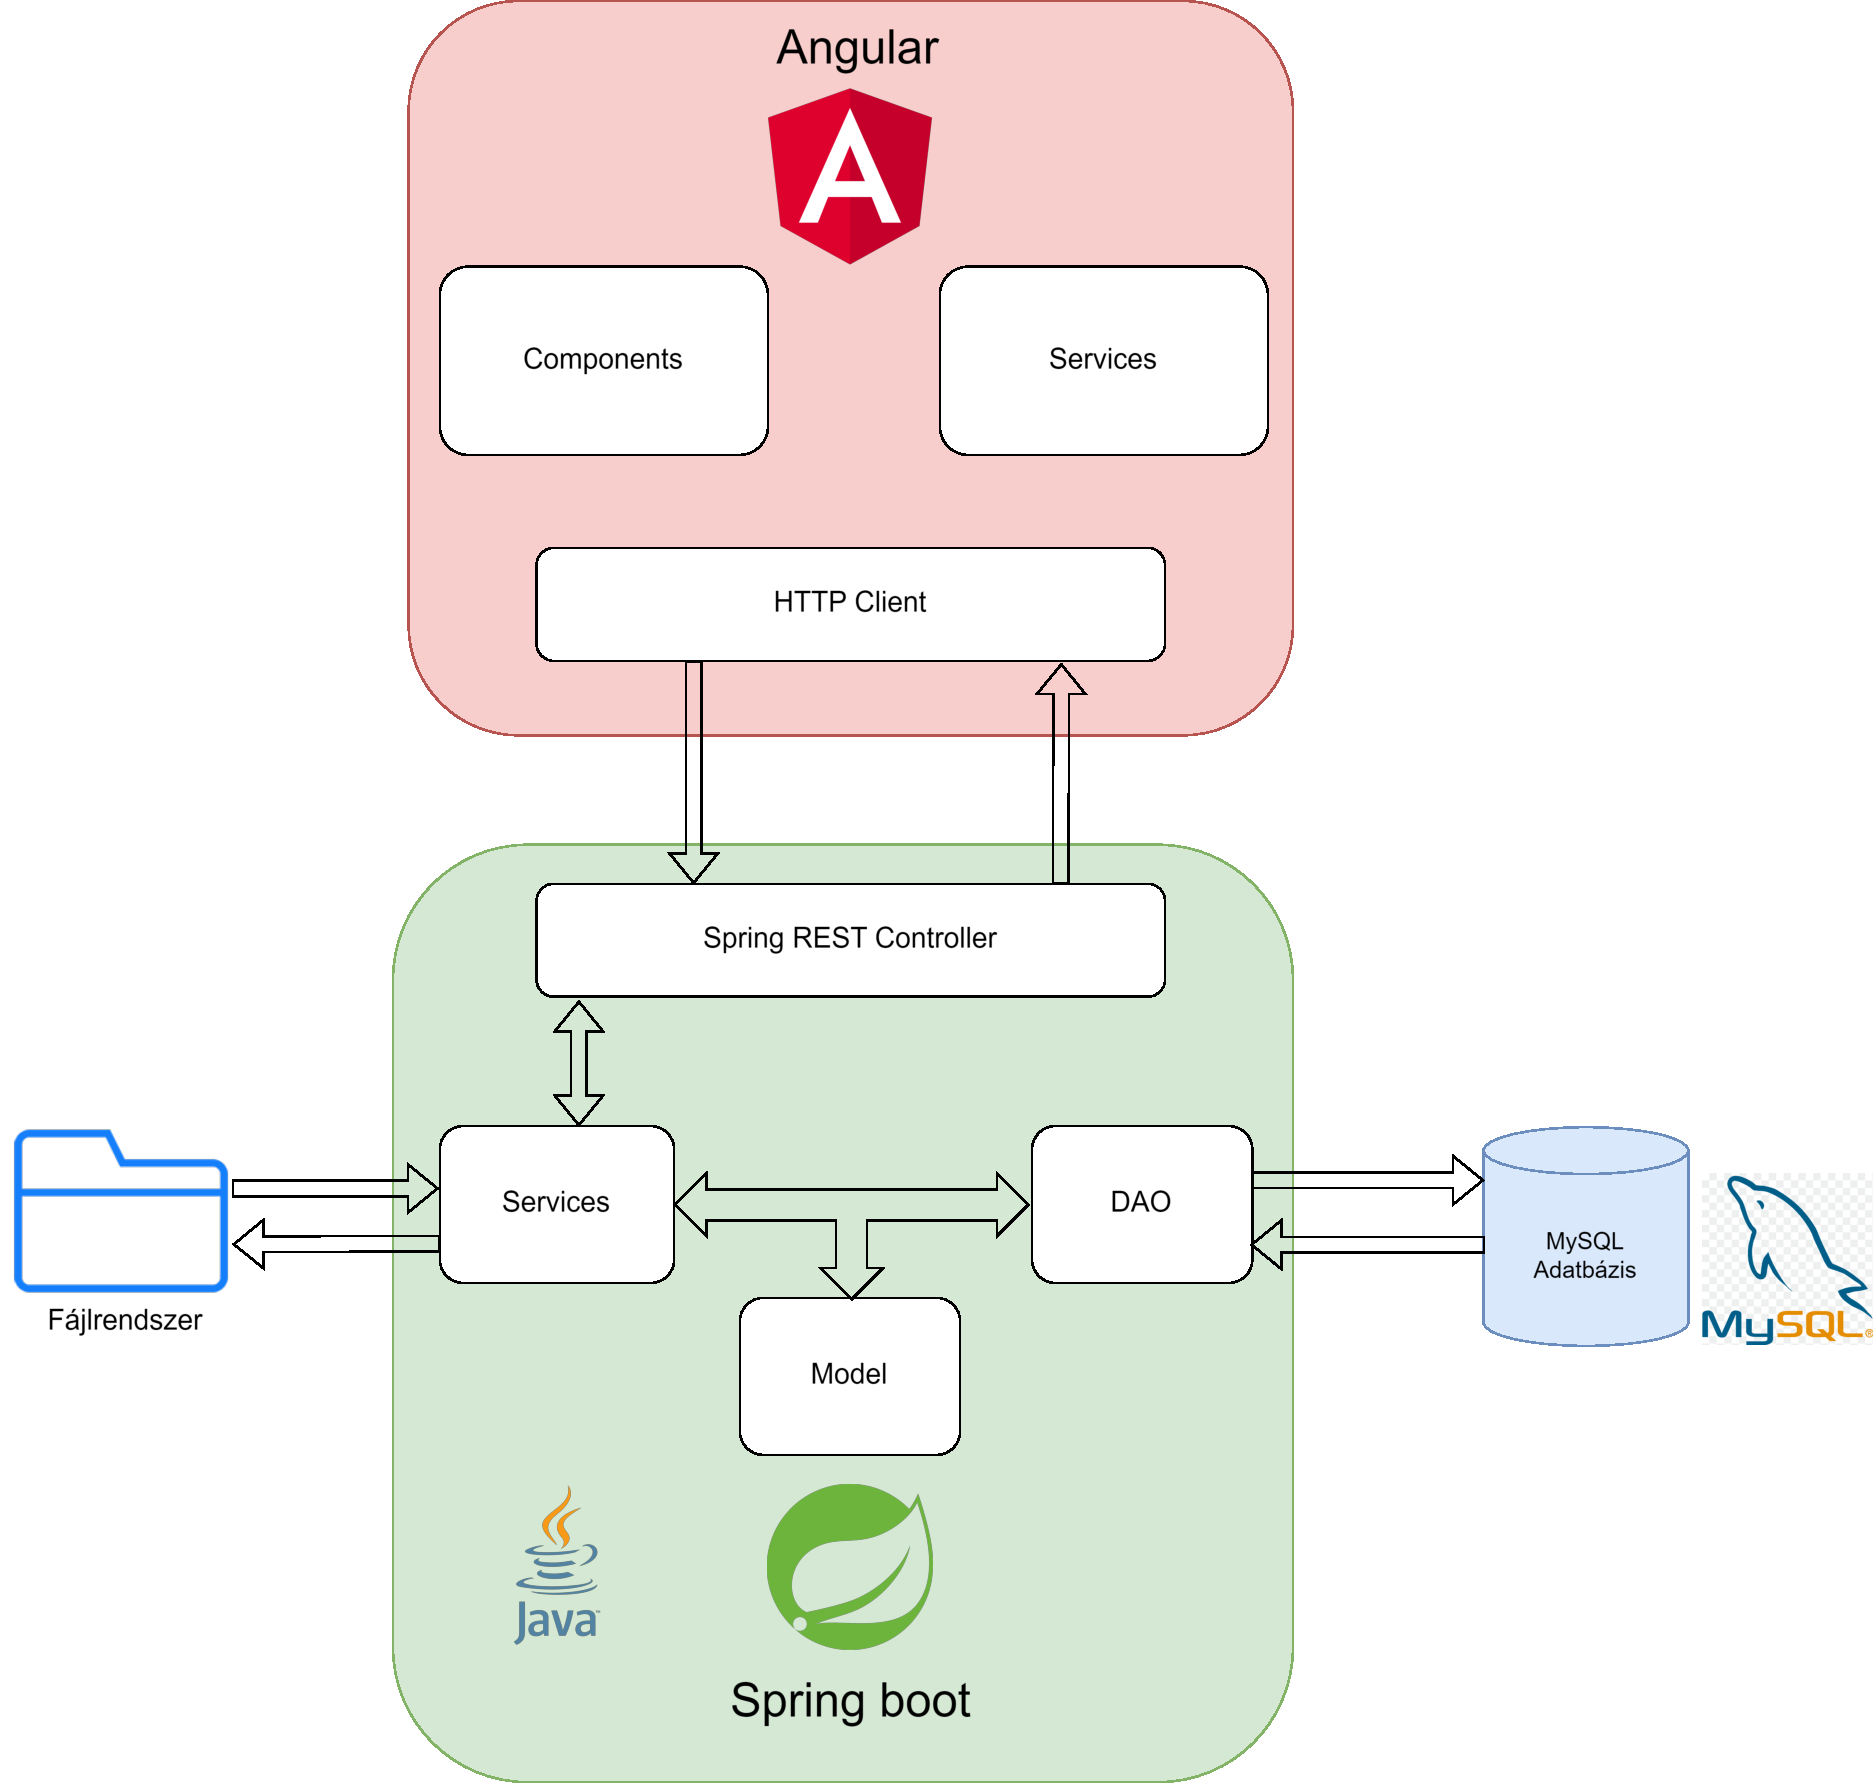
\includegraphics[width=\textwidth]{images/A_webalkalmazás_felépítése.pdf}
\caption{A webalkalmazás felépítése}
\label{fig:felepites}
\end{figure}

\Section{Perzisztens tárolás}

% Fájlrendszer: a dolgozatok, bírálatok, ... helye, tárolása, névkonvenciók.

% Adatmodellről annyit, hogy relációs séma szerint lesz, relációs adatbázissal később.

A webalkalmazás fájlrendszere a dolgozatok, prezentációk, bírálatok, záróvizsga jegyzőkönyvek illetve tételek, és e-mailek tárolását szolgálja. Az alkalmazásban a fájlok tárolásához különböző jegyzékstruktúrákat használok  fájltípusok szerint. A fájlok elérésének szempontjából az alkalmazás egyedi azonosítót (továbbiakban: 'id') és Univerzálisan Egyedi Azonosítót (továbbiakban: 'uuid') használ. Az id az adatbázisban tárolt entitások egyedi azonosítója, míg az uuid egy véletlenszerűen generált, egyedi azonosító, amelyet a fájlokhoz rendelek. Használhattam volna csak az id-t is viszont biztonságtechnikai szempontból a uuid mellett döntöttem. Ezáltal a uuid megnehezíti az illetéktelen hozzáférést a fájlokhoz, és növeli az adatbiztonságot azáltal, hogy komplikáltabbá teszi a manuális fájl elérését. A uuid használata más szempontból is előnyösnek bizonyult: Amikor a hallgató feltölti a szakdolgozatot, az alkalmazás egy uuid-t rendel hozzá, amely garantálja, hogy a fájl neve egyedülálló legyen. Ez különösen hasznos ebben az esetben, ha az összes szakdolgozat egy közös jegyzékben található, így elkerülhető a névütközés.\\
\\
Az alábbiakban felsorolom a jegyzékstruktúrákat és az egyes fájltípusok tárolásának módját:

A dolgozatok hordozható dokumentum formátum (továbbiakban: 'pdf') és tömörített fájlformátum (továbbiakban: 'zip') kerülnek tárolásra. A fájlok elnevezéseiben több helyen is szerepelnek a következő adatok:

\begin{itemize}
\item \texttt{UUID}: az egyedi azonosító \texttt{XXXXXXXX-XXXX-XXXX-XXXX-XXXXXXXXXXXX} formában, ahol az \texttt{X} helyén kisbetű vagy számjegy szerepel.

\item \texttt{name}: a hallgató neve nagy kezdőbetűvel, szóközzel tagolva.
\end{itemize}

\begin{enumerate}

\item{Dolgozatok dokumentációjai (pdfs):}

A dolgozatok dokumentációját a \textit{pdfs} nevű jegyzékben tárolom. 
A fájl feltöltésekor generálódik egy uuid, mely az első részét képezi a fájl nevének, majd ezt követi a hallgató által megadott elnevezés része.

\texttt{<UUID>\_<egyedi\_fájlnév>.pdf}, melyben

\begin{itemize}

\item \texttt{Egyedi\_fájlnév}: az egyedi fájlnév amit a hallgató ad meg általában például \texttt{dolgozat}

\end{itemize}

Például: 3c39562a-fe6a-4783-9ab4-05d875017d70\_dolgozat.pdf


\item{Dolgozatok mellékletei (zip):}

A szakdolgozatok mellékleteit az \textit{attachment} jegyzékben raktározom. A fájl elnevezése ugyanaz mint a dokumentációnál.

Például: 14e18814-1246-43cc-85e9-f4443c26f54e\_dolgozat\_melléklet.zip

\item{Prezentáció (pptx):}

A prezentációk eltárolása érdekében is egy külön jegyzéket \textit{ppts} hoztam létre, amelyben a fájlok elnevezése szintén megegyezik a fentebb említett két verzióval.

Például: 653c8797-8a8e-4472-91eb-9d7175a86891\_dolgozat\_prezentációja.pptx

\item{Bírálatok (reviews):}

A bírálatokat word formátumban tárolom le egy külön \textit{reviews} jegyzékben. A fájlnév szerkezete a következő: először az "Review" szó áll, majd a feltöltés dátuma, a hallgató neve, és végül egy uuid következik:

\texttt{Review\_<date>\_<name>\_<UUID>.docx}, melyben

\begin{itemize}
\item \texttt{date}: a dátum az \texttt{YYYY\_MM\_DD} formátumban, ahol az \texttt{YYYY} az évet, a \texttt{MM} a hónapot, a \texttt{DD} a napot jelöli,


\end{itemize}

Például: Review\_2024\_03\_20\_Minta Hallgató\_2c16f8fe-8127-4795\\-827c-65690513c2cc.docx


\item{Záróvizsga Jegyzőkönyvek (zv):}

A záróvizsga jegyzőkönyveket is word formátumban tárolom a \textit{zv} jegyzékben. Az elnevezési konvenció hasonló az bírálathoz viszont a feltöltés dátuma nem jelenik meg benne.

Például: Záróvizsga\_Minta\_Hallgató\_ab2d2f15-5701-4fc4-8022-07e877c7432f.docx

\item{Záróvizsga tételek (topics):}

A záróvizsga tételeket txt formátumban tárolom a könnyebb módosíthatóság érdekében a \textit{topics} jegyzékben. A szövegfájlba beillesztettem a záróvizsga tételeket az Alkalmazott Matematikai Intézeti tanszék honlapjáról. 


\item{E-mail (email):}

Az e-maileket a \textit{email} jegyzékben txt formátumban tárolom, hogy könnyebben módosíthassam azokat. Öt különálló szöveg fájlt hoztam létre a következő célokra: elfelejtett jelszó (forgotten\_password), bíráló felkérése (request\_review), bírálati jegyzőkönyv elküldése (review), záróvizsga létrehozása (zv\_create) és záróvizsga jegyzőkönyv elküldése (zv\_report). Ezáltal könnyen kezelhetővé teszem az egyes folyamatokhoz kapcsolódó dokumentumokat.

\end{enumerate}

A perzisztens tárolás során az alkalmazás adatmodelljét relációs séma szerint terveztem meg. Ennek értelmében az adatok strukturált formában, relációs adatbázisban lesznek tárolva a későbbi hatékony lekérdezés és adatmanipuláció érdekében. A relációs adatmodell lehetővé teszi az adatok logikai kapcsolatainak és struktúrájának pontos meghatározását, amely segíti az adatok egyszerű és hatékony kezelését, valamint az adatintegritás megőrzését. Az adatmodell megtervezése során figyelembe vettem az alkalmazás üzleti logikáját és funkcióit, hogy az adatbázis struktúrája és relációi pontosan tükrözzék az alkalmazás igényeit és funkcionalitását.

\Section{Backend}

A backend rész az alkalmazás egyik kulcsfontosságú része, amely az adatok kezelését, üzleti logikájának végrehajtását és az ügyfélkérések feldolgozását végzi. Ebben a részben bemutatom az alkalmazás Data Access Object (továbbiakban: 'DAO'), Entitás , Service és Vezérlő rétegeit.

\SubSection{DAO}

A DAO\cite{DAO} réteg egy tervezési minta, amelyet szoftverfejlesztés során alkalmaznak, különösen az adatok perzisztens tárolásának és hozzáférésének kezelésére. A Spring Boot\cite{spring_boot} alkalmazásokban is gyakran használják a DAO\cite{DAO} réteget az adatbázis műveletek kiszolgálására. Néhány fő ok, hogy miért szükséges:

\begin{itemize}

\item{} A DAO\cite{DAO} réteg segít elválasztani az üzleti logikát az adathoz való hozzáférés rétegétől. Ezáltal könnyebbé válik a kód karbantarthatósága és kiterjeszthetősége. 

\item{} Az üzleti logika nem közvetlenül függ az adatbázis technológiájától vagy a konkrét adatmodelltől, ami könnyebb tesztelést és kód újrafelhasználást tesz lehetővé. 

\item{} A DAO\cite{DAO} réteg lehetővé teszi az adatbázis műveletek optimalizálását. 

\item{} Ha az adatbázis vagy az adatmodell változik, a DAO\cite{DAO} réteg módosítása ezt a változást kezelheti, anélkül hogy az üzleti logikát érintené. 

\item{} Ha az alkalmazásnak későbbiekben változnia kell az adatbázis technológiájában (pl. MySQL-ről PostgreSQL-re), a DAO\cite{DAO} réteg könnyen cserélhető anélkül, hogy az alkalmazás más részeiben jelentős módosításokat kellene végrehajtani.

\end{itemize}

A webalkalmazásban található SQL query-k olyan mezőket kérnek le egyes táblákból, amelyek az adott lekérdezéshez szükségesek lehetnek. Azokra az adatokra amelyekre nincs szükség egy adott lekérdezés során a 'null as' kulcsszóval látom el.\\
\\
A Spring JDBC Template-t\cite{JdbcTemplate} is használhatom az SQL lekérdezések végrehajtására, és ennek segítségével is könnyedén érhetem el az adatbázist. A JDBC templatet viszont a service osztályban valósítom meg.


% Lehet ezekhez is osztálydiagram

\SubSection{Entity}

\begin{figure}[ht]
	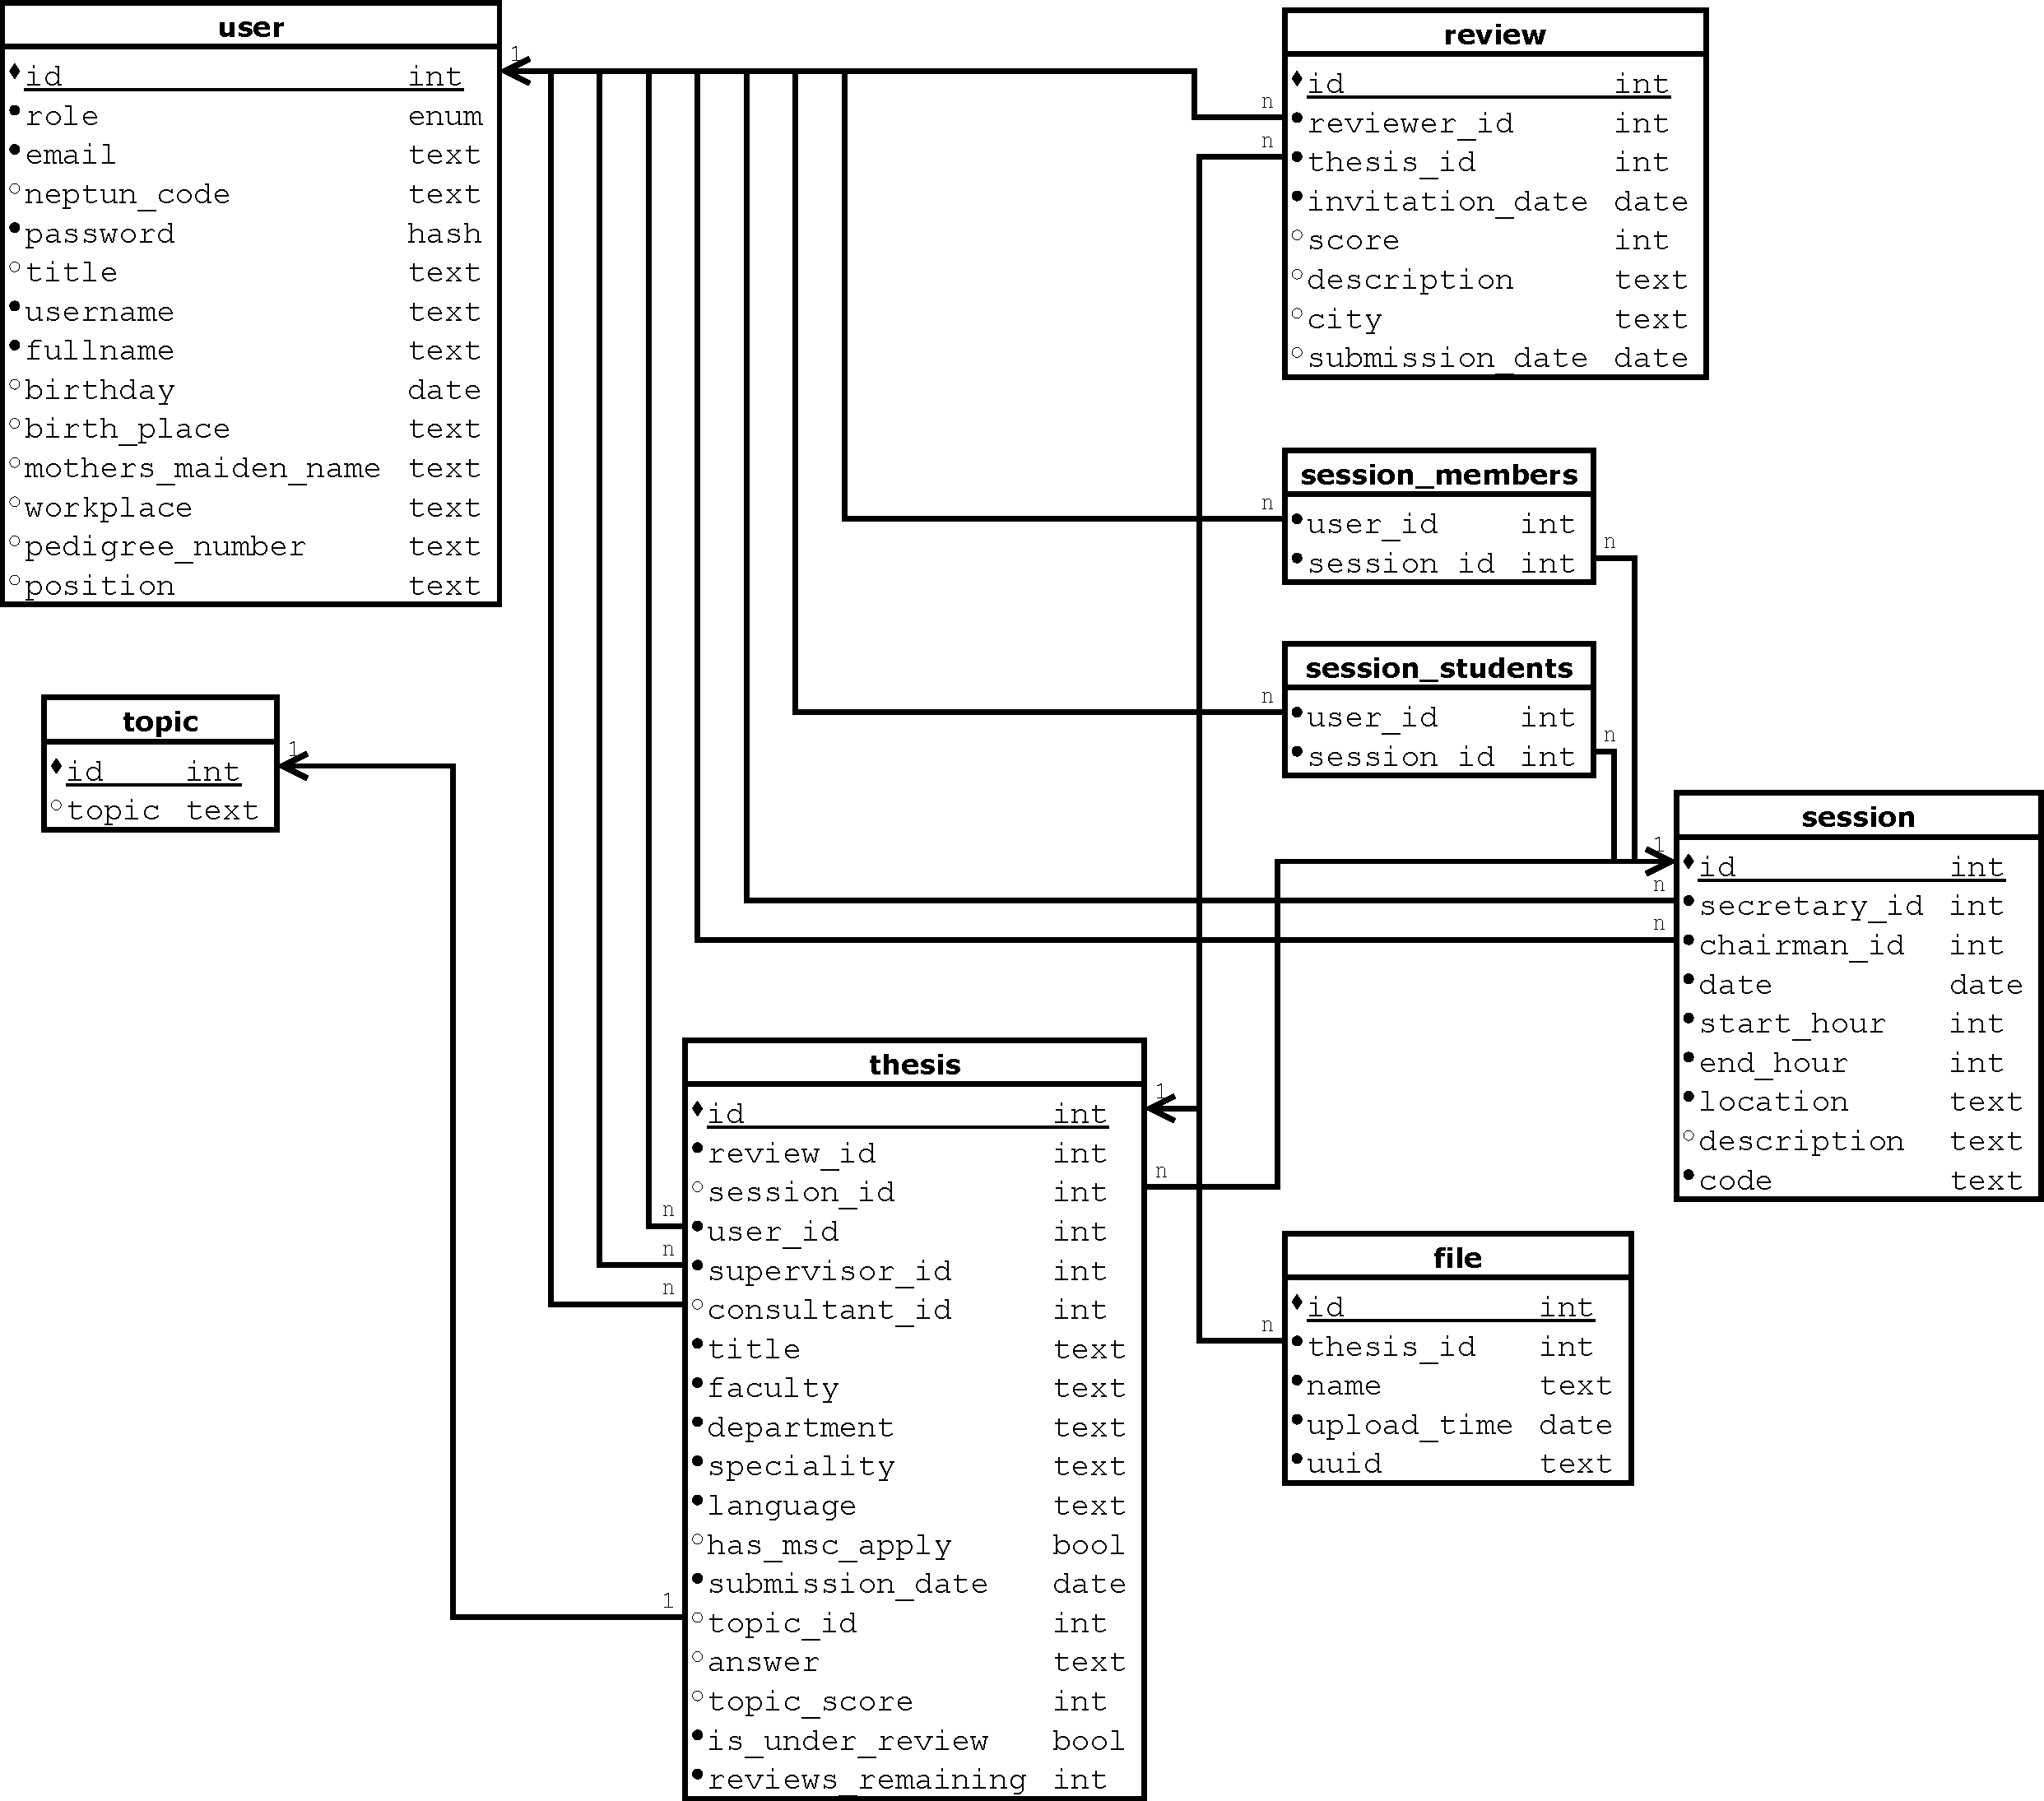
\includegraphics[width=\textwidth]{images/Adatmodell.pdf}
	\caption{Az alkalmazás adatmodelljének sémája}
	\label{fig:datamodel}
\end{figure}


Először létrehoztam a Java\cite{java} osztályokat az adatbázistáblákhoz, amelyeket JPA entitásokként definiáltam. Ezek az osztályok reprezentálják az adatbázistáblákat és tartalmazzák a tábla attribútumait. Konfiguráltam a Spring Boot\cite{spring_boot} alkalmazást, hogy csatlakozzon az adatbázishoz és használja a JPA-t az adatok kezelésére. Ehhez a application.properties fájlban megadtam az adatbázis kapcsolódási információit és konfigurációit. A Spring Data JPA segítségével Repository interfészeket hoztam létre, amelyek a JPA entitásokhoz kapcsolódnak. Ezek a interfészek kiterjesztik a Spring Data CrudRepository vagy JpaRepository interfészeket, amelyek előre definiált adatműveleteket nyújtanak az entitásokhoz. Minden entitás osztályra alkalmaztam az @Entity annotációt, hogy jelezzem, hogy az adott osztály egy JPA entitás, és kapcsolódik egy adatbázistáblához.


Minden entitáshoz létrehoztam getter-setter metódusokat az attribútumok kezelésére és beállítására, valamint egy toString metódust az objektumok olvasható formában történő megjelenítésére.

\subsubsection{User}

A \textit{User} entitásban vagyis a User.java fájlban található a felhasználó osztály. Ebben az osztályban határozom meg, hogyan kerülnek az adatok a \textit{User} táblába az adatbázisban. Az \textit{id} mező az adatbázisban az egyedi azonosítókat tárolja, amelyek segítségével azonosítani lehet egy adott felhasználót a rendszerben. Ezt a mezőt az adatbázis automatikusan generálja a "GenerationType.AUTO" stratégiát alkalmazva. A többi entitás azonosító mezőjénél is a "GenerationType.AUTO" stratégiát használom az elsődleges kulcs generálásához. A \textit{User} entitás kapcsolatban áll a \textit{Thesis}, a \textit{Review} és a \textit{Session} táblákkal. A \textit{role} mező egy enum attribútum, amely lehetővé teszi a különböző felhasználói szerepkörök (például adminisztrátor, hallgató stb.) könnyebb azonosítását és kezelését az alkalmazásban. A \textit{username}, a \textit{fullname} és az \textit{email} segíti a felhasználók azonosítását és kommunikációját az alkalmazásban. A \textit{neptun\_code}, \textit{birthday}, \textit{birth\_place}, \textit{mothers\_maiden\_name} és a \textit{pedigree\_number} mezők hozzájárulnak a hallgató könnyebb beazonosításához, valamint elengedhetetlen adatok lesznek később a záróvizsga jegyzőkönyv generálásához. A \textit{workplace}, a \textit{title} és a \textit{position} a többi szerepkör meghatározásához járulnak hozzá. A \textit{password} mező tárolja a felhasználó jelszavát, amelyet az adatbázisban hash-elt formában tárolok, így a tényleges jelszavak nem láthatóak a rendszerben.


\subsubsection{Thesis}

A \textit{Thesis} entitás az alkalmazásban olyan információkat tárol, amelyek az egyetemi hallgatók által írt szakdolgozatokra vonatkoznak. Az \textit{id} mező a \textit{Thesis} táblában egyedi azonosítót jelöl, amely segíti az adatbázisban tárolt szakdolgozatok egyértelmű azonosítását és kezelését. A \textit{Thesis} tábla összeköttetésben áll az adatbázisban szereplő összes entitással. A \textit{session\_id} mező egy idegen kulcs, amely a \textit{Session} tábla \textit{id} mezőjére mutat. A két tábla között egy-több kapcsolat áll fenn, mivel egy záróvizsgához több szakdolgozat is tartozhat. A relációt Java-ban a @ManyToOne és @OneToMany annotációval valósítottam meg. A kapcsolatot a @JoinColum annotációval egy mezőre képeztem le ez esetben ez a \textit{session\_id} mező lenne. Az idegenkulcsok kezelése hasonló a fent bemutatott példához más entitásoknál is. A \textit{user\_id}, \textit{supervisor\_id} és a \textit{consultant\_id} mezők is idegenkulcsok melyek a \textit{User} tábla \textit{id} mezőjére mutatnak. Itt is egy-több kapcsolatot valósítottam meg, mivel egy hallgatónak, témavezetőnek és konzulensnek lehet több szakdolgozata. A \textit{topic\_id} adattag a \textit{Topic} tábla \textit{id} mezőjére mutat és egy-több kapcsolatot implementáltam itt is. A \textit{title}, \textit{faculty}, \textit{department}, \textit{speciality}, \textit{language}, \textit{has\_msc\_apply}, \textit{submission\_date}, \textit{answer} mezők a szakdolgozatok könnyebb beazonosítására szolgálnak. Az \textit{is\_under\_review} a folyamatban lévő bírálatokat szeretné reprezentálni, míg a \textit{reviews\_remaining} mező a hátralévő bírálatokat tartja számon, amely alapesetben beállításra kerül 2-es értékkel.

\subsubsection{Topic}

A \textit{Topic} entitás a záróvizsgán húzott tételeket tartalmazza. Az \textit{id} mező a \textit{Topic} táblában egyedi azonosítót jelöl, amely a tétel sorszámát tárolja. A \textit{topic} mezőben pedig a záróvizsga tételek szöveges formátumban találhatóak meg. Ennél szükség volt a String típusnál nagyobb kapacitásra, mivel a záróvizsga témák leírása ennél hosszabb. Ennek megfelelően a \textit{topic} attribútum típusát VARCHAR(7500) karakterre növeltem, hogy elegendő helyet biztosítsak a témák részletes leírásához.

\subsubsection{Review}

Az \textit{Review} entitás az alkalmazásban az egyetemi szakdolgozatok értékeléseit tárolja. A szakdolgozat értékeléseket különböző szempontok alapján történik, és ezeket az adatokat rögzítem az entitásban. A táblában az \textit{id} egyedi azonosítóként szerepel. A \textit{reviewer\_id} egy idegenkulcs, amely a \textit{User} tábla \textit{id} mezőjére mutat és egy-több kapcsolatot hoztam ehhez létre. A \textit{thesis\_id} mező szintén egy idegenkulcs, amely a \textit{Thesis} tábla \textit{id} mezőjére mutat. Emellett az \textit{invitation\_date}, \textit{score}, \textit{description}, \textit{city} és \textit{submission\_date} mezők szolgálnak az értékelések egyértelmű azonosítására és részletezésére. A \textit{description} mező esetében felmerült az adatméret korlátozottsága, ezért a @ColumnDefinition annotáció segítségével kiküszöböltem a problémát, beállítva a mező típusát LONGTEXT-re, ezáltal lehetővé téve a bírálatok részletes leírásának tárolását.

\subsubsection{File}

A \textit{File} entitás az alkalmazásban a fájlok tárolását szolgálja a szakdolgozatokhoz és egyéb kapcsolódó dokumentumokhoz. Az \textit{id} mező a \textit{File} entitásban egyedi azonosítóként szolgál, amely segíti az adott fájl egyértelmű azonosítását az adatbázisban. A \textit{thesis\_id}-t idegenkulcsként hoztam létre amely a \textit{Thesis} tábla \textit{id} mezőjével áll kapcsolatban. Egy-több kapcsolatot valósítottam meg, mivel egy szakdolgozathoz több fájl is rendelhető. A \textit{name}, \textit{upload\_time} és \textit{uuid} mezők a fájlok egyértelműbb beazonosítására szolgálnak. A \textit{uuid}, ahogy a perzisztens tárolásnál említettem segít elkerülni az azonos nevű vagy azonos tartalmú fájlok ütközését, valamint könnyen lehetőséget nyújt az adatok azonosítására és kezelésére.

\subsubsection{Session}

A \textit{Session} entitás az alkalmazásban a záróvizsgák adatait tárolja. Az \textit{id} mező a \textit{Session} entitásban egyedi azonosítóként szolgál, amely lehetővé teszi az adott záróvizsga egyértelmű azonosítását az adatbázisban. A \textit{secretary\_id} és a \textit{chairman\_id} idegenkulcsok, amelyek segítségével könnyen beazonosítható a jegyző és az elnök személye. A \textit{members} és a \textit{students} külön táblákba hoztam létre, mivel több-több kapcsolatot valósítottam meg a \textit{User} és a \textit{Session} entitás között. A két táblában a felhasználó és a záróvizsga azonosítóját tárolom. A \textit{date}, \textit{start\_hour}, \textit{end\_hour}, \textit{location}, \textit{description} és a \textit{code} adattagok a záróvizsgák egyértelműbb beazonosítására szolgálnak illetve ezek a záróvizsga jegyzőkönyv generálásához elengedhetetlen adattagok.

\newpage
\subsection{Service}

A Spring Boot alkalmazásban a Service osztályok általában az üzleti logika rétegét képviselik. Ezek az osztályok felelősek az üzleti folyamatok végrehajtásáért, adatfeldolgozásért és egyéb műveletekért, amelyeket az alkalmazás végrehajt.

\subsubsection{UserService}

A UserService osztály a felhasználók kezeléséért és az ahhoz kapcsolódó műveletek végrehajtásáért felelős. Az addUser metódus lehetővé teszi, hogy új felhasználót adjunk hozzá az adatbázishoz. Itt beállítottam, hogy a jelszó hash-elt formában kerüljön be az adatbázisba, felhasználva a getEncodedPassword metódust. Az updateUsers metódussal felülírhatjuk a felhasználók egyes adatait. A user-t megkapom frontendről és annak az egyedi azonosítója alapján lehet frissíteni az egyes adattagokat. Ha a felhasználó szerepköre hallgató akkor beállítottam, hogy a beosztás mező üres legyen. A deleteUserbyId metódussal törölhetünk felhasználót az egyedi azonosítója alapján az adatbázisból. Ezenkívül létrehoztam különböző metódusokat, amelyek az adott felhasználók beazonosítására szolgálnak. Így meg tudjuk őket jeleníteni egy táblázatban illetve a drop-down listában is. A felhasználók beazonosíthatóak név, egyedi azonosító és szerepkör alapján.
Ezekhez felhasználom a dao rétegben írt lekérdezéseket, amelyek segítségével biztosítom az adatok védelmét. A findStudentsByLoggedInReviewer függvényre a Thesis status lap miatt van szükség, mivel szerettem volna úgy elkészíteni az oldalt, hogy a bíráló és a témavezető is csak azt a hallgatót lássa, akinek bírálatot kell írni. Az init metódusokkal inicializálok különböző szerepkörökből felhasználókat azért, hogy amikor elindul az alkalmazás ezek már létrejöjjenek azonnal. Ez sokban segítette néhány funkció tesztelését, hogy nem kellett mindig létrehozni felhasználót, szakdolgozatot stb.-t hogy egyből ki tudjak próbálni egy új funkciót. A jelszóváltoztatást segítő metódusokat is itt hoztam létre. Készítettem először is egy getEncodedPassword metódust, amelyben használom a PasswordEncoder osztály passwordEncoder metódusát annak érdekében, hogy a jelszó titkosítva legyen hash formátumban az adatbázisban.

\subsubsection{ThesesService}

A ThesesService osztály felelős a szakdolgozatokkal kapcsolatos műveletek végrehajtásáért és az azokhoz kapcsolódó adatbázis-műveletek kezeléséért. Az addTheses updateTheses és a deleteThesesbyId metódusok funkciója nem tér el a userService-ben látottakhoz képest annyi, hogy most szakdolgozatokkal végezhető el ez a művelet. Itt is megtalálhatóak különböző metódusok, amelyek a szakdolgozat pontos beazonosítására szolgálnak akár egyedi azonosító alapján és a felhasználó egyedi azonosítója alapján is.

\subsubsection{TopicService}

A TopicService osztály felelős a záróvizsga tételekkel kapcsolatos műveletek végrehajtásáért és az azokhoz kapcsolódó adatbázis-műveletek kezeléséért. Az addTopics metódus segítségével új záróvizsga tételt lehet hozzáadni egy szakdolgozathoz. A chooseTopic eljárásban valósítottam meg egy jdbcTemplattel a tételhúzást. Amikor a felületen megtörténik a folyamat, akkor az adatbázisban a Thesis tábla topic\_id és topic\_score mezője frissül. A getTopics metódussal egy listába kapom vissza a záróvizsga tételeket. Az initTopics metódussal inicializálom a tételeket. Ezeket egy tömbben tárolom el. Azért mert amikor újból indítom az alkalmazást akkor mindig legenerálódik ismételten a 27 db tétel ezért írtam rá egy sql querry-t, amely megszámolja hogy mennyi szakdolgozat van és ha még nincs szakdolgozat akkor inicializálja a tételeket.

\subsubsection{FileService}%%%%%%%%%%%%%assemblewithstudent-et át kell írni backenden

A FileService felelős a fájlok kezeléséért, beleértve a feltöltést, letöltést, fájlnevek lekérdezését és törlését. Az assembleFileWithThesis metódus összerendezi a fájlt a megadott szakdolgozattal. Ellenőrzi, hogy a fájl és a szakdolgozat megtalálható-e az adatbázisban. Ha megtalálhatóak, akkor hozzárendeli a fájlt a szakdolgozathoz. A findThesesByLoggedInStudent metódus az éppen a rendszerbe belépett felhasználó egyedi azonosítóját kapja meg. Ez alapján végig iterál a szakdolgozatokon és vizsgálja, hogy az adott dolgozathoz tartozik-e fájl, ha nem akkor a fájlfeltöltéses felületen megjelenik az adott felhasználó szakdolgozata a legördülő listában. A getFilenameByUUID metódus az adatbázisból keresi és visszaadja a fájl nevét a uuid alapján. Erre fájl letöltésnél van szükség. A getFile metódus visszaadja a fájlt a megadott fájlnév alapján. A deleteFileById metódus uuid alapján töröl az adatbázisból fájlokat. Az uploadFile metódussal feltölti a felhasználó a megadott fájlt. A fájl típusától függően megfelelő mappákba menti a fájlt, és beállítja a fájl nevét és egyéb adatait az adatbázisban.

\subsubsection{EmailSenderService}

Ez az osztály felelős az e-mail küldés funkcióért, amihez egy külön e-mail címet hoztam létre. Először is hozzáadtam a pom.xml fájlban a megfelelő függőséget. Utána létrehoztam egy mailConfiguration, amely egy konfigurációs osztály. Ebben az osztályban létrehoztam a getJavaMailSender metódust, amelyben beállítom a JavaMailSenderImpl példányát, amely a tényleges e-mail küldésért felelős. Ebben megadom a Gmail SMTP szerver adatait, valamint az SMTP hitelesítéshez szükséges felhasználónevet és jelszót.Ezután létrehoztam egy emailSenderService osztályt, ahol az e-mail küldést valósítottam meg. A sendEmailWithAttachments metódus egy olyan e-mailt küld, amelynek van csatolmánya. A paraméterei a címzett e-mail címe (toEmail), a levél tárgya (subject), a levél szövege (body) és a csatolt fájl elérési útvonala (pathToAttachment) amelyet String típusú listában adtam meg. Ez a metódus létrehoz egy MimeMessage objektumot, amelyet a JavaMailSender segítségével állít be. A csatolt fájlt a FileSystemResource segítségével adja hozzá a levélhez. Ha a csatolt fájl nem található, akkor kivételt dob. Végül a mailSender.send(message) hívással elküldi az e-mailt, majd a konzolra kiírja, hogy sikeresen kiküldésre került az e-mail. A sendEmail metódus egy olyan e-mailt küld, amelynek nincs csatolmánya. Paraméterei ugyanazok, mint a sendEmailWithAttachment metódusnak, csak itt nincs pathToAttachment paraméter. A funkciója ugyanaz, csak csatolmány nélkül küldi el az e-mailt.

\subsubsection{ForgottenPasswordService}

Ez az osztály kezeli az elfelejtett jelszóval és a beállításával kapcsolatos folyamatokat, például az új jelszó kérést és az e-mailen keresztüli jelszóvisszaállító token küldését. A forgottenPasswordToken metódus egy felhasználóhoz generál egy jwt tokent, amelyet a felhasználó e-mailben fog megkapni. Ezt beállítottam hogy 10 percig legyen érvényes. Az isValidPassword metódus az új jelszó beállításához szükséges. Az új jelszó megadásához meg kell adni a régit is ezt ellenőrzi ez a metódus. Az elfelejtett jelszó eseténél létrehoztam egy isValidToken metódust is, ami a megadott tokent, hogy az egyezik-e az e-mailben kiküldöttel. A setNewPassword metódus lehetővé teszi a felhasználó számára, hogy új jelszót állítson be a kapott token segítségével. Ellenőrzi, hogy a token érvényes-e, majd megváltoztatja a felhasználó jelszavát a megadott újra. A setNewPasswordtwo metódus lehetővé teszi a felhasználó számára, hogy új jelszót állítson be a régi jelszóval. A sendForgottenPasswordTokenByEmail metódus egy e-mailt küld a felhasználónak, amely tartalmazza a jelszóvisszaállító token-t. Az e-mail tartalmazza a token-t és egy leírást, hogy meddig érvényes a token. Ha a felhasználó nem található meg a megadott felhasználónév alapján, akkor egy UsernameNotFoundException kivételt dob.

\subsubsection{JWT alapú autentikáció és azonosítás kezelése}

JWT alapú autentikációs és azonosítási rendszer kifejezetten fontos szerepet tölt be az alkalmazásban, biztosítva a felhasználók biztonságos hozzáférését és azonosítását. JwtRequest és JwtResponse osztályok az autentikációs kérés és válasz objektumokat reprezentálják. A JwtRequest tartalmazza a felhasználónevet és a jelszót, míg a JwtResponse tartalmazza a felhasználót és a JWT tokent. Az autentikációs problémák érdekében létrehoztam egy külön osztályt amely kezeli az autentikációs hibákat. Amennyiben a kliens nem rendelkezik megfelelő hitelesítő adatokkal vagy érvénytelen tokent küld, a rendszer HTTP 401 Unauthorized választ küld vissza. A JwtRequestFilter osztályban amikor egy kérés érkezik, kinyeri belőle a JWT tokent a fejlécből, majd ellenőrzi annak érvényességét. Ha a token érvényes, akkor beállítja a felhasználói azonosítást a Spring Security SecurityContextHolder objektumban. A WebSecurityConfiguration konfigurációs osztály konfigurálja a Spring Security-t. Beállítja, hogy mely végpontok érhetők el mindenki számára, és melyek csak hitelesített felhasználók számára. Hozzáadja a JwtRequestFilter-t a Spring Security láncolatához. A JwtService szolgáltatásosztály felelős az autentikációs folyamat teljes körű kezeléséért. Itt valósul meg a felhasználók azonosítása, az autentikáció során a JWT tokenek generálása és validálása. 


\subsubsection{ReviewService}

A ReviewService a bíráló és a témavezető által készített bírálatok kezeléséért felelős a rendszerben. Az addReview metódus felel a bírálatok adatbázisba mentéséért. Itt külön beállításra kerülnek a remaining\_review és az is\_under\_review mezők amelyek a még hátra lévő és a folyamatban lévő bírálatokat kezelik. A getReviewData metódus a bírálatok kigyűjtésére szolgál. A findThesesByUserIdAndReviewerId metódus a szakdolgozatokat keresi meg témavezető és bírálói azonosító alapján. Ez hasonló okok miatt lett létre hozva mint a findThesesByUserId metódus a FileService-ben. A findReviewByThesisId metódus a szakdolgozat egyedi azonosítója alapján keresi meg a bírálatot. A Proba metódusban történik a bírálat word dokumentummá generálása. Itt először hozzáadtam a megfelelő függőséget a pom.xml-ben. A felhasználó amint megadja az adatokat kliensoldalon az elmegy a szerver felé, ami feldolgozza ezeket az adatokat és ezek alapján egy word dokumentumot készít. A metódus paraméterként egy objektumot kap, amely tartalmazza a bírálat részleteit. Az objektumot String formátumra alakítja, majd feldolgozza és kinyeri belőle a szükséges információkat, mint például a hallgató nevét, a dolgozat címét, a bíráló nevét, a bírálat részletes leírását stb. Az Apache POI segítségével létrehoz egy üres Word dokumentumot.
Beállítja a dokumentum fejlécét, amely tartalmazza az egyetem nevét és logóját. Beilleszti a dokumentumba a felhasználók által megadott információkat, mint például a hallgató nevét, a dolgozat címét, a bíráló nevét, a bírálatot stb. Ezeket a részleteket formázott szövegként adja hozzá a dokumentumhoz. A generált Word dokumentumot elmenti egy kijelölt könyvtárba. A fájlnevet a dokumentumhoz kapcsolódó adatokból generálja, például a hallgató nevét és egy uuid-t is tartalmazza. A metódus elmenti a generált Word dokumentum adatait az adatbázisba. Az adatbázisban tárolja a fájl nevét, feltöltési idejét és egyedi azonosítóját, hogy később könnyen visszakereshető legyen. A fájl mentése után a Word dokumentum generálása során számos formázási lehetőséget alkalmazok a szöveg és egyéb elemek megjelenítéséhez. Ezek közé tartozik a setText, setFontSize, setFontFamily metódusok használata, amelyekkel beállíthatom a szöveg stílusát, betűméretét és betűtípusát. Emellett lehetőségem van új bekezdéseket létrehozni addBreak a szöveg tagolásához, valamint képeket is beilleszthetek a dokumentumba. A táblázatokat is könnyedén formázhatom, például a cellák méretét vagy szegélyeit állíthatom be. Emellett a táblázatok celláinak láthatóságát is szabályozhatom, hogy megfeleljenek az adott formai követelményeknek. Ezen funkciók segítségével teljes körűen testreszabhatom és formázhatom a generált Word dokumentumokat, hogy azok megfeleljenek az elvárásoknak és esztétikusak legyenek. A táblázatok esetében létrehoztam egy külön függvényt a méretük beállítására. Ennek köszönhetően könnyen változtathatom a táblázatok méretét az alkalmazás különböző részein.

\subsubsection{GenerateDocxService}

A generateDocxService osztály felelős a záróvizsga jegyzőkönyv generálásáért. A függvény egy Object típusú paramétert kap ugyanúgy, majd ebből a paraméterből kinyeri a szükséges adatokat, mint például a hallgató nevét, a szakdolgozat címét, a bizottság tagjainak adatait stb. Ezeket az adatokat felhasználva létrehoz egy Word dokumentumot, amelyben formázott módon jeleníti meg a jegyzőkönyvet. A dokumentumban címeket, bekezdéseket, táblázatokat és egyéb formázott szövegeket helyez el a megfelelő helyeken a jegyzőkönyv struktúrájának megfelelően. A végeredmény egy Word fájl lesz, amely tartalmazza a generált záróvizsga jegyzőkönyvet.

\subsubsection{SessionService}

A SessionService a Session entitással kapcsolatos üzleti logikát valósítja meg. A findSessionById metódus lehetővé teszi egy záróvizsga entitás keresését az azonosító alapján. Az addSessions metódus a záróvizsga felvitelét végzi el. Először lementi a záróvizsgát az adatbázisba, ezután e-maileket küld az összes érintett félnek (tagok, hallgatók, elnök, jegyző, stb.) az emailSenderService osztály sendEmail metódus segítségével. A további metódusok arra szolgálnak, hogy az eddigi záróvizsgákat lekérjük a rendszerből.

\subsubsection{StatusService}

A StatusService a szakdolgozatok állapotának kezelésével és azokhoz kapcsolódó folyamatok végrehajtásával foglalkozik. A getNeccessaryData metódus lekéri azokat az adatokat, amelyek szükségesek a szakdolgozatok állapotának és azokhoz kapcsolódó folyamatoknak a kezeléséhez. Ez a metódus a Thesis Statuts és Report Status felületek miatt lett létrehozva. A metódus lefuttatja a megfelelő adatbázis-lekérdezést a FileDao segítségével, majd feldolgozza az eredményeket és visszaadja egy listában. A findFilesByThesesId metódus megkeresi egy adott szakdolgozathoz tartozó bírálatokat és azokat elküldi egy e-mailben a hallgatónak. Először lekéri a megfelelő szakdolgozatot az azonosítója alapján. Ezután lekéri a szakdolgozathoz tartozó hallgató adatait és a kinyert e-mail címre elküldi a szakdolgozathoz tartozó bírálatokat egy e-mailben.


\subsubsection{ReportstatusService}

A ReportStatusService a szakdolgozatok állapotának jelentésével kapcsolatos üzleti logikát valósítja meg. A requestForReview metódus a bírálónak küld felkérést egy szakdolgozat bírálatra. A bíráló felkérése után rögtön e-mail megy ki a bírálónak benne a szakdolgozat címével. Ezután a szakdolgozat állapota az is\_under\_review mezőben megváltozik igaz értékre. A findThesesUnderReview metódus visszaadja az összes olyan szakdolgozatot, amely jelenleg bírálat alatt áll, azaz az is\_under\_review mező értéke igaz. Ez lehetővé teszi a rendszer számára, hogy kezelje és megjelenítse ezeket a szakdolgozatokat a jegyző és az elnök számára. A findReviewedTheses metódus visszaadja az összes olyan szakdolgozatot, amely már átesett a bírálaton. 


\subsection{Vezérlők}

% Kontrollernek is hívják.

A vezérlő osztályok a Spring keretrendszerben az alkalmazás üzleti logikájának és az HTTP kérések kezelésének központi pontjai. Ezek az osztályok felelősek a bejövő HTTP kérések fogadásáért, feldolgozásáért és a megfelelő válasz létrehozásáért. A vezérlő osztályok a @RestController annotációval vannak ellátva, és HTTP kéréseket kezelő metódusokat tartalmaznak, melyek különböző útvonalakra vannak mappelve. A vezérlő osztályok meghatározzák az alkalmazás által kezelt útvonalakat. Ezek az útvonalak az HTTP kérésekhez vannak hozzárendelve, és megadják, hogy mely metódusokat kell meghívni az adott kérésre érkező adatok kezelésére. A vezérlő osztályok fogadják és feldolgozzák a bejövő HTTP kéréseket. Ezek a kérések lehetnek GET, POST, PUT, DELETE stb. típusúak, és a megfelelő metódusok hívódnak meg azok kezelésére. Például GET kérésekkel lekérdezhetők a felhasználók adatai, POST kérésekkel új felhasználók hozhatók létre, PUT kérésekkel módosíthatók a felhasználók adatai, DELETE kérésekkel pedig törölhetők a felhasználók. A TopicsController részben használtam még egy PostConstruct annotációt is. A @PostConstruct annotációval ellátott metódus az osztály példányosítása után hívódik meg. Ebben az esetben a initTopics() metódus meghívása történik, amely a topicService inicializálását és beállítását végzi el. Ez azért fontos, mert biztosítja, hogy a témák inicializálása megtörténjen a TopicsController példányosítása után, még mielőtt bármely más kérést kezelnénk a controllerben. A vezérlő osztályok hívják az service réteget, hogy végrehajtsák az alkalmazás üzleti logikáját. Ez lehet adatok lekérdezése, módosítása vagy más üzleti folyamatok végrehajtása. A vezérlő osztályok felelősek a megfelelő válasz létrehozásáért az adott HTTP kérésre. Ez lehet HTML oldal renderelése (ha a @Controller annotációt használjuk), vagy JSON válasz küldése (ha a @RestController annotációt használjuk). A vezérlő osztályok gyakran végzik az adatok validációját, és kezelik a különböző hibákat, amelyek a HTTP kérések feldolgozása során jelentkezhetnek.\\
\\
A rendszerben összesen kilenc vezérlő osztályt hoztam létre, melyek mindegyike különböző funkciókat lát el és kezeli a kapcsolódó HTTP kéréseket. Ezek a vezérlők az alábbiak:
\begin{itemize}

\item{UsersController}
\item{ThesisController}
\item{FileController}
\item{GenerateDocxController}
\item{JwtController}
\item{ReportStatusController}
\item{ReviewController}
\item{SessionController}
\item{TopicsController}

\end{itemize}

\begin{figure}[ht]
	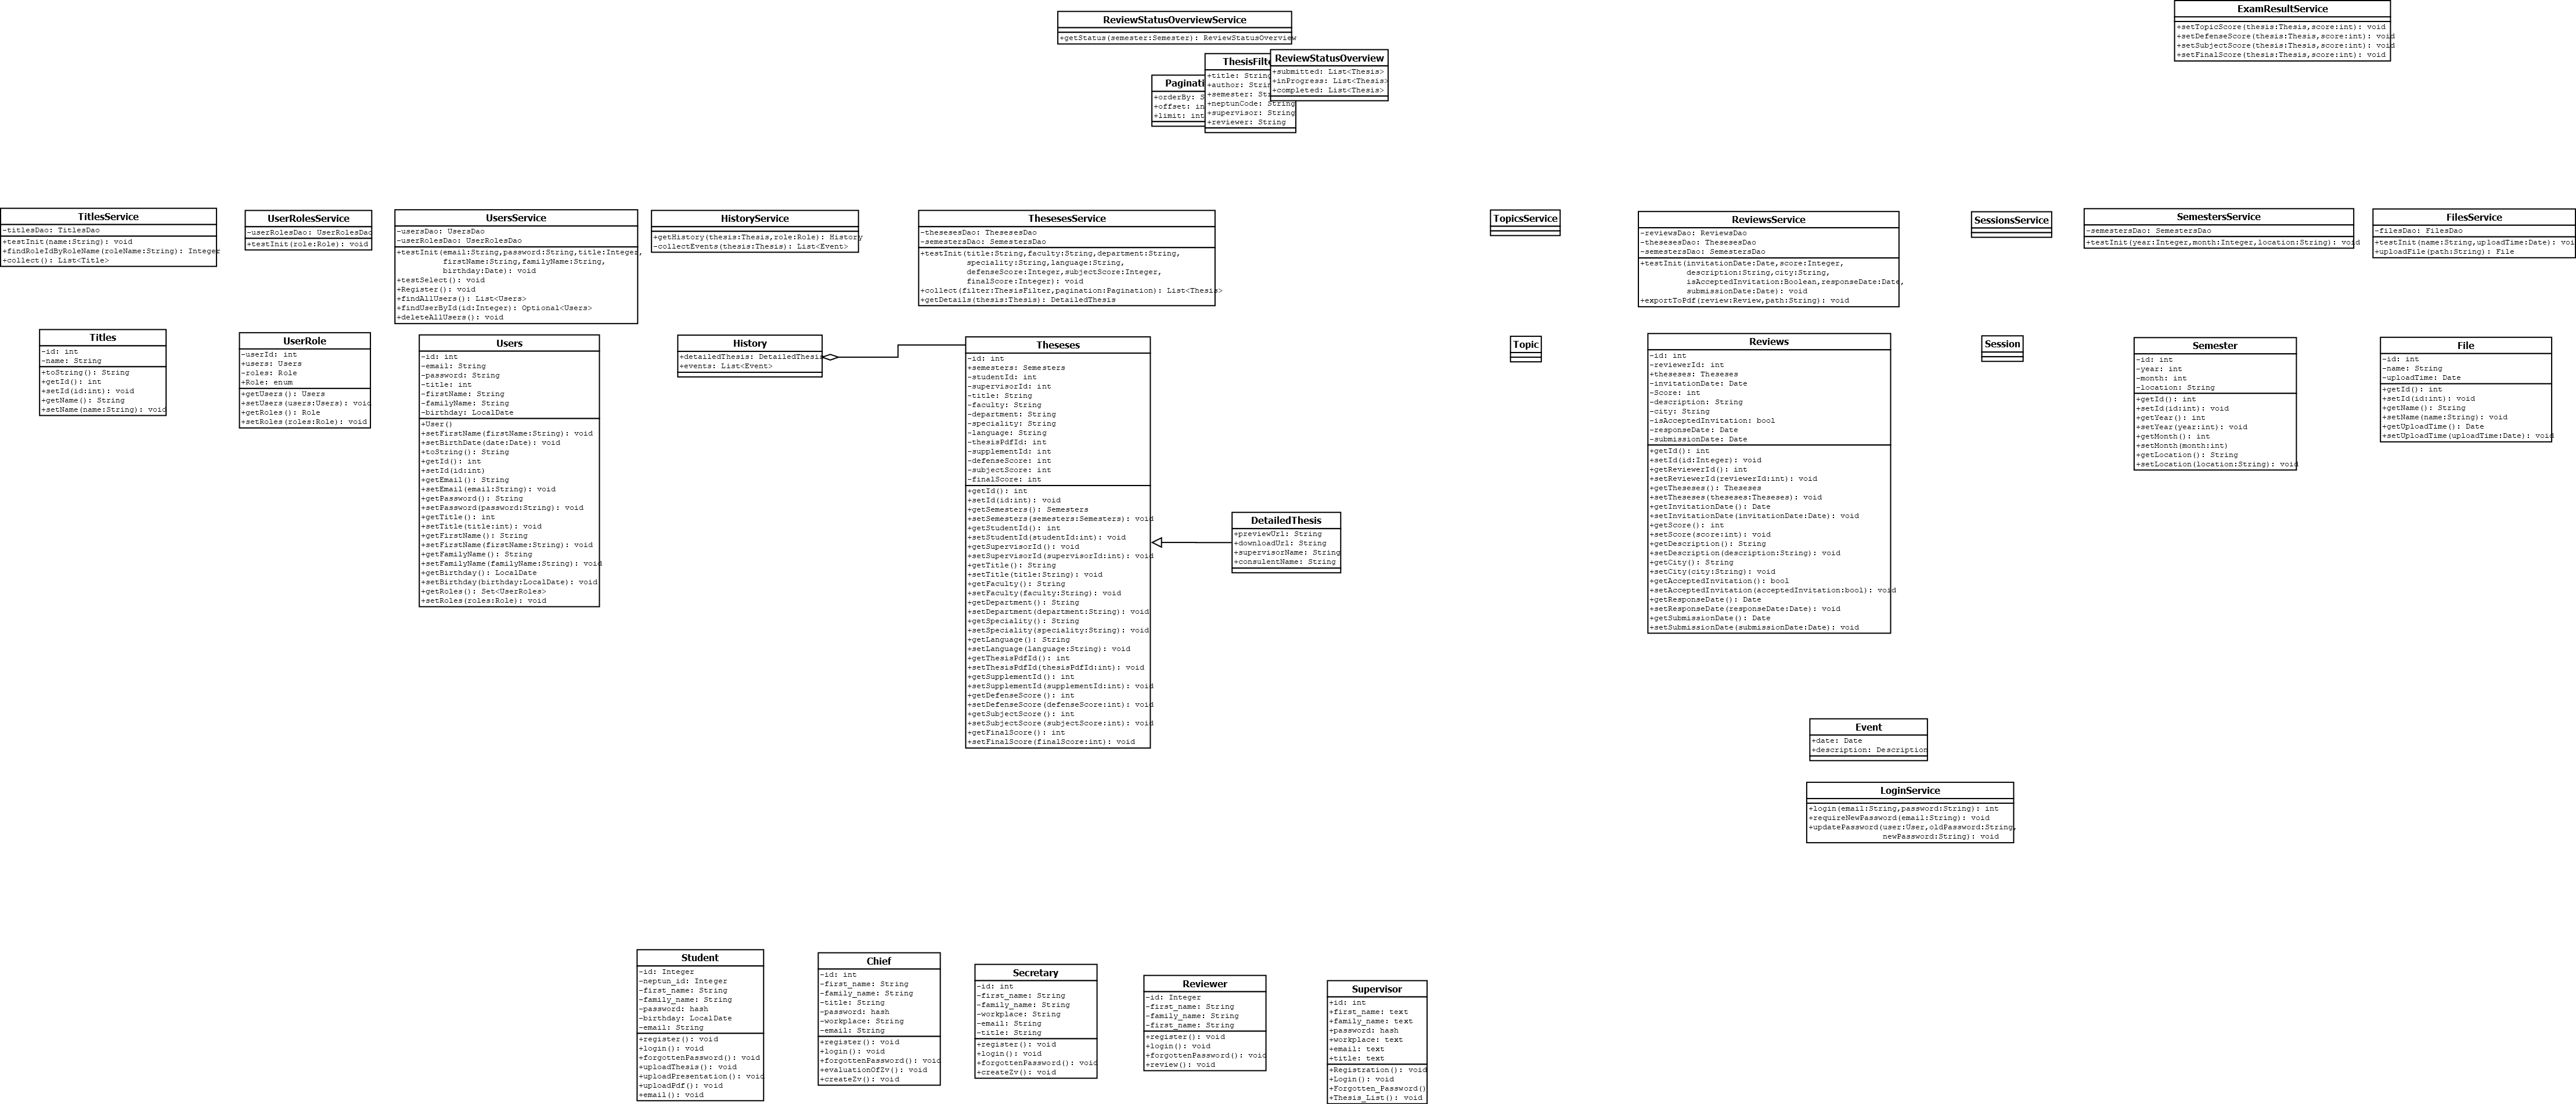
\includegraphics[width=\textwidth]{images/Osztálydiagram.pdf}
	\caption{Az alkalmazás osztálydiagramjának részlete}
	\label{fig:Osztálydiagram}
\end{figure}



\Section{A REST API áttekintése}

A Representational State Transfer Application Programming Interface (továbbiakban: REST API)\cite{REST API} egy olyan szoftveres architekturális stílus, amelyet webes szolgáltatások kialakítására használnak. Az API-k különböző platformokon keresztül teszik lehetővé az alkalmazások közötti kommunikációt. A REST API-k\cite{REST API} az erőforrásokat (pl. adatbázis rekordokat) reprezentálják és kezelik, a HTTP\cite{http} protokoll különböző metódusainak (GET, POST, PUT, DELETE stb.) segítségével.

A backend és frontend összekapcsolása úgy történik, hogy a backend kiszolgálja az adatokat a frontend felé, amely a felhasználói felületet megjeleníti és a felhasználó interakcióit kezeli. Ezt úgy valósítják meg, hogy a frontend kliens oldalon HTTP\cite{http} kéréseket indít a backend felé, amelyekre a szerver válaszol.\\

Itt láthatjuk hogy az egyes kéréstípusokhoz például milyen REST API végpontok tartoznak:

\begin{enumerate}

\item{\textbf{GET:}}
A GET kérések általában adatok lekérésére szolgálnak. Például, a backend a /getThesesListToDisplay végpontján keresztül teszi elérhetővé a szakdolgozatok listáját a frontend számára. Ezenkívül, a frontend a /findThesesById végpontot is használhatja egy adott szakdolgozat részleteinek lekérésére egyedi azonosító alapján.

\item{\textbf{POST kérés:}}
A POST kérések új adatok beküldésére szolgálnak a szerver számára. Például, a frontend az /addThesis végpontra küldheti a felhasználó által hozzáadni kívánt dolgozat adatait. A backend a kapott adatok alapján hozzáadja az új szakdolgozatot az adatbázishoz, majd visszaküldi az új tézist a frontendnek.

\item{\textbf{PUT:}}
A PUT kérések meglévő adatok frissítésére szolgálnak a szerveren. Például, a frontend az /updateThesis végpontra küldheti a felhasználó által szerkesztett szakdolgozat adatait. A backend frissíti az adatbázisban a megfelelő thesis rekordot az új adatokkal, majd visszaküldi a frissített dolgozatot a frontendnek.

\item{\textbf{DELETE kérés:}}
A DELETE kérések adatok törlésére szolgálnak a szerveren. A frontend a /deleteThesis végpontra küldheti a felhasználó által törölni kívánt szakdolgozat azonosítóját. A backend az egyedi azonosító alapján törli az adatbázisból a szakdolgozatot.

\end{enumerate}


\Section{Frontend}

Az Angular\cite{angular} frontend fejlesztésének középpontjában a komponensek és servicek állnak. A komponensek az alkalmazás felhasználói felület részeit képviselik, míg a szolgáltatások központosítják az alkalmazás logikáját és funkcionalitását. A frontend fejlesztés során ezeket az építőköveket kombinálom, hogy részletes és felhasználóbarát webalkalmazást hozzak létre.

Elsőként szeretném bemutatni az alkalmazás fő modulját. Az AppModule egy Angular\cite{angular} modul, amely felelős az alkalmazás fő komponenseinek, szolgáltatásainak és moduljainak konfigurálásáért és összekapcsolásáért. \\
\\Fontos tulajdonságai:

\begin{itemize}

\item{Deklarációk:} A declarations tömbben felsorolom az összes komponenst és direktívát, amelyeket az alkalmazásban használok. Ezek közé tartoznak például a felhasználó felvitele, záróvizsga létrehozása stb. komponensek. 

\item{Importálások:} Az imports tömbben felsorolom azokat a modulokat, amelyeket az alkalmazás használ. Ezek között találhatók a Ng2OrderModule (a rendezésért felelős modul), AppRoutingModule (az alkalmazás útvonalainak kezeléséért felelős modul), NgxPaginationModule (a lapok számozásáért felelős modul) és a HttpClientModule (a HTTP\cite{http} kérésekhez szükséges modul), valamint más modulok, például az Angular Material moduljai.

\end{itemize}

Az AppRoutingModule egy külön modul, amely a fő alkalmazás útvonalait kezeli. A RouterModule.forRoot(routes) segítségével konfigurálom az alkalmazás útvonalait a routes tömb segítségével, ahol minden útvonalhoz megadom, hogy melyik komponenshez tartozzon. Ez azért fontos, mert az Angular\cite{angular} útvonalak segítségével navigálja a felhasználókat az alkalmazásban.

% Angular Service-ek bemutatása.

\subsection{Servicek}

Az Angular\cite{angular} service-ek olyan osztályok, amelyek segítenek a frontend alkalmazás és a szerveroldali  szolgáltatások közötti adatátvitelben és kommunikációban. Az Angular alkalmazások gyakran kommunikálnak a szerverrel, hogy adatokat kérjenek, frissítsenek vagy mentsenek. Ehhez az Angular\cite{angular} service-ek HTTP\cite{http} kéréseket hajtanak végre a backend API felé, például GET, POST, PUT vagy DELETE kéréseket küldenek a szervernek a szükséges adatokkal. Ezenkívül az Angular\cite{angular} szolgáltatások lehetővé teszik az adatok megosztását és átvitelét a különböző komponensek között is. Például egy szolgáltatásban tárolt adatokat egy vagy több komponens használhatja, ami lehetővé teszi az alkalmazás különböző részeinek adatainak szinkronizálását és koherenciáját.\\
\\Ezekből 12 darabot hoztam létre:

\begin{itemize}

\item{AddDocxService}
\item{AddFileService}
\item{AddSessionService}
\item{AddThesisService}
\item{AddTopicService}
\item{AddUserService}
\item{AuthService}
\item{DocumentService}
\item{FindAllUserService}
\item{ListThesisService}
\item{ReportStatusService}
\item{LoginService}

\end{itemize}

% Template-ek.

\subsection{Komponensek}

Az Angular alkalmazásokban a komponensek az építőkövek, amelyek létrehozzák az alkalmazás felhasználói felületét és meghatározzák, hogy az hogyan viselkedik és milyen módon reagál a felhasználói interakciókra. A komponensek négy fő részből állnak: a TypeScript (.ts) fájlból, a spec TypeScript (.spec.ts) fájlból, a HTML fájlból és a CSS fájlból. A TypeScript fájl a komponens logikáját és viselkedését definiálja, míg a spec TypeScript fájl a komponens teszteléséhez szükséges specifikációkat tartalmazza. Az HTML fájl tartalmazza a komponens megjelenítéséhez szükséges struktúrát és sablonokat, míg a CSS fájl a stílusokat és formázást definiálja a komponens számára. A TypeScript és a HTML fájlok interaktív felhasználói felületet biztosítanak, míg a CSS fájl az esztétikai megjelenést és a formázást szabályozza. A komponensek felelősek az adatok megjelenítéséért, a felhasználói interakciók kezeléséért és az alkalmazás üzleti logikájának koordinálásáért.\\
\\
Ezekből 18-at hoztam létre:

\subsubsection{AddUsersComponent}

Az AddUsersComponent egy Angular komponens, amely felelős a felhasználók felviteléért az alkalmazásban. Ebben a komponensben a felhasználókhoz kapcsolódó adatokat gyűjtöm össze és továbbítom az AddUsersService szolgáltatáshoz. Az adatok felvitelénél különös figyelmet szenteltem, hogy az egyes szerepkörök esetén a beosztás mező csak az adott szerepkörrel rendelkező felhasználókhoz jelenjen meg. Ennek érdekében hoztam létre az onRoleChange függvényt. Az adatok helyes felvitelét validatorok segítségével oldottam meg, ahol létrehoztam egyedieket is, annak érdekében hogy ne kelljen minden mezőt minden szerepkör esetén kitölteni. Az e-mail validációját egy reguláris kifejezéssel, vagy regexszel oldottam meg. A regex egy olyan szövegmintázat, amely lehetővé teszi a szövegben való keresést vagy illesztést egy meghatározott mintához. Ez a reguláris kifejezés ellenőrzi, hogy az e-mail cím megfelelő formátumú-e a következő szerkezet szerint: felhasznalonev@domain.com. A helyes form beküldés esetén sweetalert2 csomag importálásával dizájnos figyelmeztető szöveget helyeztem el. Amennyiben a felhasználó nem megfelelő jogosultsággal rendelkezik, a komponens nem jeleníti meg az oldalt, hanem figyelmeztetést ad a felhasználónak, majd átirányítja a bejelentkező oldalra. Ezt az ngOnInit függvényben állítottam be, ahol egy roleMatch függvény alapján vizsgálom az éppen bejelentkezett felhasználót, hogy jogosultságot kaphat-e az oldalhoz. Amennyiben nem, továbbirányítom egy másik oldalra. Ezt a folyamatot minden lapnál elvégeztem.\\
\\A komponens HTML része:\\
\\
Az adatok felviteléhez egy container-t hoztam létre, amely tartalmazza az űrlapot. Az űrlap egy card elemen belül található, ami további stílusokat ad az űrlaphoz. Az ngSubmit eseményvezérlő a form küldésekor hívódik meg, és a addFormData függvényt hívja meg az űrlap értékeivel. A [formGroup] direktíva az addUserForm FormGroup-hoz köti az űrlapot, amely a ts fájl-ban lett definiálva. A formon belül a mezők formControlName direktívával kapcsolódnak a FormGroup-hoz. Az input mezők, választógombok és dátumválasztók mellett használok *ngIf strukturális direktívát is, hogy a mezők csak bizonyos feltételek teljesülésekor jelenjenek meg. Betekintést nyertem az Angular Material használatába, amely lehetővé teszi számomra, hogy az alkalmazásban modern és összhangban lévő felhasználói felületet hozzak létre. Az űrlap alján egy gomb található, amely a form elküldésére szolgál, és csak akkor aktív, ha az űrlap érvényes állapotban van. 

\subsubsection{AddThesesesComponent}

Az AddThesesesComponent egy Angular komponens, amely felelős a szakdolgozatok felviteléért az alkalmazásban. Ez a komponens funkcióját tekintve megegyezik az előzővel. Létrehoztam külön függvényeket a drop-down listákhoz amelyek role alapján kiválogatják a témavezetőket, hallgatókat és konzulenseket.  Az űrlap tartalmaz mezőket a szakdolgozat címéhez, tanszékhez, specializációhoz, nyelvhez, hallgatóhoz és témavezetőhöz. Az űrlap ugyanúgy validációval rendelkezik, és csak a megfelelő adatok megadása esetén engedi a form elküldését. Az addFormData függvény az űrlap adatait elküldi a szervernek, majd megjeleníti a sikeres üzenetet, és átirányítja a felhasználót a fájlfeltöltés oldalra. Ha hiba történik az adatok küldése közben, akkor hibaüzenet jelenik meg a felhasználónak.\\
\\
A komponens HTML része:\\
\\
Az AddThesesesComponent HTML részletében ugyanúgy egy űrlapot hoztam létre, amely lehetővé teszi a felhasználó számára, hogy új szakdolgozatot adjon hozzá a rendszerhez. Az űrlap strukturált módon felépített, és tartalmazza a szükséges mezőket a szakdolgozat részletes leírásához. A mezők kötelező kitöltését ellenőrző validációk biztosítják, hogy a felhasználó csak akkor tudja elküldeni az űrlapot, ha minden szükséges adatot helyesen megadott. Amennyiben valamelyik mező hiányos vagy hibás adatot tartalmaz, a felhasználót figyelmeztető szövegek jelennek meg a megfelelő mező mellett. Az űrlapot egy "Felvitel" gomb zárja, amely csak akkor aktív, ha az összes mező helyesen van kitöltve. Ezt a gombot használva a felhasználó elküldi az űrlapot, és a rendszer rögzíti az új szakdolgozat adatait.

\subsubsection{AddDocxComponent}

Az AddDocxComponent komponensben a bírálat írásának felülete került implementálásra. A komponens kezdeti betöltésekor az ngOnInit függvényen keresztül meghívja a getStudentsToDropdown metódust a bejelentkezett felhasználóhoz tartozó hallgatók lekérésére. Az űrlap tartalmaz egy lenyíló listát, amely segítségével a felhasználó kiválaszthatja a hallgatót, akinek a dokumentumot létre szeretné hozni. A hallgató kiválasztása után az onSelectStudent metódus hívásával betöltődik az adott hallgatóhoz tartozó szakdolgozat. Az űrlap egyes mezőinek kötelező kitöltését ellenőrző validációk biztosítják, hogy a felhasználó csak akkor tudja elküldeni az űrlapot, ha minden szükséges adatot helyesen megadott. Az űrlapot elküldve az addFormData metódus hívódik meg, amely létrehozza és letölti a generált dokumentumot a szerverről. Ha a letöltés sikeres volt, akkor a felhasználó értesítést kap a sikerességről, ellenkező esetben pedig hibaüzenet jelenik meg.\\
\\
A komponens HTML része:\\
\\
Az AddDocxComponent komponenshez tartozó HTML űrlap segítségével a felhasználó kiválaszthat egy hallgatót, hozzárendelhet egy szakdolgozatot, megírhatja a bírálatot egy textarean belül, valamint  egy érdemjegyet adhat a szakdolgozatra. A textareat css fájl-ban módosítottam annak érdekében hogy dinamikus legyen a méretezése a felületen.

\subsubsection{AddSessionComponent}

Az AddSessionComponent komponens a záróvizsgák hozzáadását teszi lehetővé az alkalmazásban. Ez a komponens funkcióját tekintve megegyezik az utóbbival. Az űrlap beküldését az addFormData metódus teszi lehetővé. A sikeres beküldést követően ugyanúgy egy sikeres üzenet jelenik meg, míg ellenkező esetben egy hibás üzenet. A form helyes beküldését ugyanúgy validátorok ellenőrzik. A drop-down listákat ugyanúgy külön függvényben valósítottam meg. A form elküldése után felugrik egy modal, amely figyelmezteti a felhasználót az e-mailek kiküldésére.\\
\\
A komponens HTML része:\\
\\
A html kód hasonló az előzőekhez. Amikor a felhasználó rányom a submit gombra meghívódik a waiting függvény, amíg az e-mailek kiküldésre kerülnek.


\subsubsection{AuthComponent}

Az auth.guard.ts fájl tartalmaz egy AuthGuard nevű osztályt, amely egy átfogó szolgáltatás, és implementálja a CanActivate interfészt. Ennek a célja, hogy ellenőrizze a felhasználó be van-e jelentkezve az alkalmazásba, és rendelkezik-e a megfelelő jogosultságokkal az adott útvonal eléréséhez. Ha a felhasználó be van jelentkezve és rendelkezik a megfelelő jogosultságokkal, akkor az útvonal elérhető lesz számára, különben hibaüzenetet kap. Az auth.interceptor.ts fájl egy HTTP interceptor-t tartalmaz, amely az összes HTTP kérést megelőzi. A célja, hogy hozzáadja a JWT tokent az autorizációs fejléchez minden olyan kérésben, amely nem rendelkezik a No-Auth fejléccel. Ezenkívül a catchError operátor segítségével az interceptor figyeli a válaszokat, és kezeli az esetleges hibákat. Ha a válasz státuszkódja 401 vagy 403, a felhasználót a megfelelő helyre irányítja, és megjeleníti a megfelelő hibaüzenetet.


\subsubsection{FindAllUsersComponent}

A FindAllUsersComponent nevű komponens felelős az összes felhasználó megjelenítéséért és kezeléséért. A komponens feladatai közé tartozik az összes felhasználó lekérése, a keresés funkciók megvalósítása, a felhasználók szerkesztése és törlése. A findAllUsers metódus segítségével a komponens inicializálásakor az összes felhasználó adatát lekéri és megjeleníti a rendszer. A keresési funkciók, mint például searchForStudent, searchForNeptunCode, searchForEmail, searchForWorkplace, lehetővé teszik a felhasználók szűrését az adott kritériumok alapján.  Az updateUsers metódus segítségével a felhasználók adatait frissíthetjük, és a deleteUser metódus segítségével törölni lehet a kiválasztott felhasználót. Az onRoleChange metódus a felhasználói szerepkör változását figyeli, és beállítja a megfelelő megjelenítést a pozíció mezőnek. Bíráló esetén input mező, témavezető, jegyző és elnök esetén pedig legördülő listát adtan hozzá a megjelenítéshez. Az adatok rendezését és oldalankénti megjelenítését is kezelem a key, reverse és p változók segítségével. Az alertWithError metódus figyeli és kezeli az esetleges hibákat, és megjeleníti a megfelelő hibaüzenetet.\\
\\
A komponens HTML része:\\
\\
A html kódban a kereséseket containerekben helyeztem el. A felhasználók adatait egy táblázatban jelenítem meg, ahol az oszlop fejlécénél lehetőség van rendezni is az adatokat. A táblázat fejléce után beállítom hogy egy lapon hány felhasználó szerepeljen. A táblázathoz külön hozzáadtam még két gombot, amelyek az adott felhasználó adatainak módosítására és törlésére szolgálnak. A módosítást egy felugró modal-ban implementáltam.


\subsubsection{HeaderComponent}

A Header komponens felelős a navigációs sáv megjelenítéséért az alkalmazásban. Az isLoggedIn metódus visszaadja, hogy a felhasználó be van-e jelentkezve vagy sem. A bejelentkezési állapotot a AuthService szolgáltatás isLoggedIn metódusa alapján határozza meg. A logout metódus felelős a felhasználó kijelentkeztetéséért. Először meghívja a AuthService clear() metódusát, amely törli a felhasználó adatait a bejelentkezési tárolóból. Ezután átirányítja a felhasználót a főoldalra a Router segítségével.\\
\\
A HTML kódban a navigációs sáv megjelenítése, a bejelentkezés és kijelentkezés gomb elhelyezése van implementálva.


\subsubsection{ListSessionsComponent}

Ez a komponens a listázza a záróvizsgákat Az AddSessionService segítségével lekéri a záróvizsgák adatait. Az ngOnInit metódusban hívódik meg a listSessions metódus, amely betölti és megjeleníti a záróvizsgákat. A resp változón végigiterálok és elvégzem a dátum formázáshoz szükséges teendőket. Az adatok rendezését és oldalankénti megjelenítését is kezelem a key, reverse és p változók segítségével.\\
\\
A komponens HTML része:\\
\\
A html kódban egy táblázatban jelenítem meg a záróvizsgák adatait.  A hallgatók és a tagok listája egy belső span elemmel van megvalósítva, hogy megfelelően megjelenítsem a hallgatók és tagok nevét, valamint az utolsó elem után ne jelenjen meg vessző. A pagination-controls elem az oldalszámok megjelenítését biztosítja a lapozószámként.

\subsubsection{ListThesesesComponent}

A komponens listázza a szakdolgozatok adatait. A getThesesList segítségével lekéri a szakdolgozatok listáját a megjelenítéshez. Itt ugyanúgy végigiterálok a resp változón és elvégzem a dátum helyes formázását. Felhasználók által megadott kritériumok alapján lehetőséget biztosítok a szakdolgozatok keresésére cím, beküldési dátum és hallgató neve alapján. A jegyző itt adhatja meg, hogy a hallgató milyen tételt húzott a záróvizsgán és hogy milyen érdemjegyet kapott rá. Lehetőséget biztosítok a szakdolgozatok szerkesztésére és törlésére az adatbázisból. A szakdolgozat módosításánál ugyanúgy legördülő lista segítségével változtathatjuk meg a hallgatót, a témavezetőt és akár a konzulenst is. A szakdolgozat törlésére is lehetőség van amelyre a deleteTheses függvényt hoztam létre. Lehetőség van a táblázatban megjelenő szakdolgozatok rendezésére. \\
\\
A komponens HTML része:\\
\\
A html kódban a kereséseket ugyanúgy containerek segítségével hoztam létre.
Külön kihívást nyújtott a dátum alapján keresés, amelyet a datepicker segítségével oldottam meg. Az adatokat ugyanúgy egy táblázatban jelenítem meg, ahol lehetőség van rendezésre. Ezenkívül elhelyeztem gombokat a módosítás, törlés és tétel húzás funkciókhoz is. A táblázatban a kitöltetlen adatokat kiküszöböltem egy *ngif direktívával és írtam egy elseBlock-ot. A módosítást és a tétel húzást egy felugró ablakban valósítottam meg. Ahol input mezőket date-pickert és legördülő listát is volt alkalmam alkalmazni.


\subsubsection{LoginComponent}

A LoginComponent komponens a felhasználó bejelentkezésének folyamatát kezeli az  alkalmazásban. A alertWithNewPassword függvény egy értesítést jelenít meg a felhasználónak a sikeres jelszóváltoztatásról. Az alertWithUnauth függvény figyelmeztetést ad a felhasználónak, ha az autentikáció nem sikerült (HTTP 401 hibakód). Az alertWithWrongPassword függvény célja, hogy ha a megadott jelszó helytelen (HTTP 500 hibakód). A login függvény felelős a felhasználó bejelentkezéséért. Elküldi a bejelentkezési adatokat a UserService szolgáltatásnak, majd a válasz alapján továbbítja a felhasználót a megfelelő oldalra. A forgottenPw függvény az elfelejtett jelszó funkcióját kezeli. Elküldi a felhasználó által megadott felhasználónév alapján az e-mailt. A changePw függvény a jelszóváltoztatás funkcióját kezeli. Elküldi az új jelszót és az ellenőrző kódot a UserService szolgáltatásnak, majd értesíti a felhasználót a sikeres jelszóváltoztatásról. A matchPwValidator egy egyedi validációs függvény, ami ellenőrzi, hogy az új jelszó és a megerősítő jelszó egyezik-e a jelszóváltoztatás folyamatában.\\
\\
A komponens HTML része:\\
\\
Egy űrlap a bejelentkezéshez, amely tartalmazza a felhasználónév és jelszó mezőket, valamint egy bejelentkezés gombot. Van egy gomb az "Elfelejtett jelszó" funkcióhoz, amely egy modal ablakot nyit meg. Két felugró ablak a "Elfelejtett jelszó" és "Új jelszó beállítása" funkciókhoz. A "Elfelejtett jelszó" modal ablak tartalmaz egy űrlapot a felhasználónév megadásához az új jelszó igényléséhez. Az "Új jelszó beállítása" modal ablak egy űrlapot tartalmaz a felhasználónév, token, új jelszó és az új jelszó megerősítése megadásához.


\subsubsection{MyprofileComponent}

A MyprofileComponent egy jelszóváltoztató oldalt valósít meg. A komponens meghívja a szerveroldali metódusokat és azok segítségével hajtja végre a jelszó módosítást. A jelszóváltoztatás funkcióhoz validátor is tartozik, amely ellenőrzi az új jelszó és a megerősítő jelszó egyezőségét. A módosítást egy felugró ablakban valósítottam meg.\\
\\
A komponens HTML része:\\
\\
Az HTML kód egy jelszóváltoztatás űrlapot és egy hozzá tartozó gombot tartalmaz, amely megnyitja a jelszóváltoztatás modal ablakát. A felugró ablakban található egy űrlap, ahol a felhasználó megadhatja jelenlegi és új jelszavát, valamint megerősítheti az új jelszót. Ha az új jelszó és a megerősítő jelszó nem egyezik meg, akkor megjelenik egy felhívó szöveg, amely figyelmezteti a felhasználót.


\subsubsection{ReportStatusComponent}

A ReportStatusComponent a szakdolgozatok státuszának nyomonkövetéséért felelős komponens. A komponens a jegyző és elnök szerepköröknek készült elsősorban. Három részre lehet osztani az oldalt a beadott szakdolgozatokra, a folyamatban lévő bírálatokra, és a befejezett bírálatokra. Mindháromhoz létrehoztam egy tömböt és ezekben tárolom le a szükséges adatokat. A requestForReview függvényben lehetőség van a bíráló felkérésére.A komponens különböző segédfüggvényekkel rendelkezik, például az alertWithReview, alertWithError, alertWithFileType, amelyek segítenek kezelni a különböző hibákat vagy értesítéseket. A correctTable metódusban az adatok rendszerezése és formázása történik a megfelelő megjelenítés érdekében. A komponens tartalmaz továbbá metódusokat a fájlok letöltéséhez.\\
\\
A komponens HTML része:\\
\\
A megjelenítést egy összecsukható listával valósítottam meg a három fő részre.
\\
\begin{enumerate}

\item{} Beadott szakdolgozatok: Ez a rész tartalmazza a beadott szakdolgozatok adatait egy táblázatban. A táblázat oszlopai a Neptunkód, Hallgató neve, Témavezető név, Bíráló név, Cím, Beadás dátuma és a letölthető fájlok (PDF, Melléklet, PPT). Minden sorban a szakdolgozatokhoz kapcsolódó információk találhatók, és lehetőség van a fájlok letöltésére.

\item{} Folyamatban lévő bírálatok: Ez a rész hasonlóan tartalmazza a folyamatban lévő bírálatok adatait, mint az előző rész, de csak azokat a szakdolgozatokat listázza, amelyek jelenleg bírálat alatt állnak.

\item{} Befejezett bírálatok: Ez a rész a befejezett bírálatok adatait tartalmazza. A táblázat hasonló az előző kettőhöz, de az itt felsorolt szakdolgozatokhoz már hozzá vannak rendelve a bírálatok fájljai is. Emellett lehetőség van a bírálatokhoz tartozó fájlok letöltésére és a bírálatok küldésére e-mailben.\\
\end{enumerate}
Ezeken kívül a kód egy modal komponenst is tartalmaz, amely lehetővé teszi a bíráló kiválasztását egy űrlap segítségével. A modal egy legördülő menüt tartalmaz, amelyben a bírálókat lehet választani. Az űrlap elküldése után a kiválasztott bírálóhoz küldött kérelem feldolgozásra kerül.

\subsubsection{ThesisStatusComponent}

A ThesisStatusComponent a szakdolgozatok státuszának kezelését végzi. A komponens a hallgató, bíráló és témavezető szerepköröknek készült elsősorban. Ennek a komponensnek a feladata szakdolgozatok megjelenítése és hogy mindegyik szerepkör csak a hozzá tartozó szakdolgozatokat lássa. A funkcióját tekintve hasonló az előzőhöz. Keresési funkciót is implementáltam a szakdolgozatok és  A komponens tartalmazza az adatlekéréseket és az ezekkel kapcsolatos műveleteket, például a fájlok letöltését vagy törlését, a keresést a táblázatban, valamint a felhasználói visszajelzések megjelenítését. Betölti és kezeli a szakdolgozatokhoz és felhasználókhoz kapcsolódó adatokat, valamint a szakdolgozatok fájljait. Lehetővé teszi a szakdolgozatokhoz tartozó fájlok letöltését és törlését. Biztosítja a keresési funkciót a táblázatban.\\
\\
A komponens HTML része:\\
\\
A hmtl kódban containerek-ben helyeztem el a kereséseket. Az adatokat egy táblázatba szúrtam be. Külön létre hoztam gombokat a fájlok letöltésére és törlésére is.

\subsubsection{UploadPdfZipFilesComponent}

Az UploadPDFZIPFilesComponent felelős a PDF és ZIP fájlok feltöltéséért a rendszerbe. Az onFileSelected metódus figyeli az eseményeket, amikor a felhasználó kiválaszt egy fájlt a feltöltéshez. Ez a metódus ellenőrzi a kiválasztott fájlok típusát és méretét, és megfelelő hibaüzeneteket jelenít meg, ha a kiválasztott fájlok nem felelnek meg a követelményeknek. Ha a fájlok megfelelőek, akkor tárolja azokat a megfelelő változókban a későbbi feltöltéshez. A uploadFile metódus felelős a kiválasztott fájlok feltöltéséért a szerverre. Ez a metódus létrehoz egy FormData objektumot, amely tartalmazza a kiválasztott fájlt, majd a AddFilesService segítségével elküldi azt a szervernek. A feltöltés közben figyeli a fájlok feltöltési folyamatát, és a sikeres feltöltés után összekapcsolja a fájl azonosítóját és a szakdolgozat azonosítóját a szükséges műveletek végrehajtásához. Az alert-el kezdődő metódusok felelősek különböző típusú figyelmeztetések és üzenetek megjelenítéséért a felhasználók számára a feltöltési folyamat során felmerülő eseményekről és hibákról. Végül a komponens tartalmaz egy getTheses metódust is, amely a bejelentkezett felhasználóhoz kapcsolódó szakdolgozatokat kéri le a szerverről a ListThesesesService szolgáltatás segítségével, és azokat tárolja a theses változóban a későbbi felhasználásra.\\
\\
A komponens HTML része:\\
\\
Az HTML kód arra szolgál, hogy lehetővé tegye a felhasználók számára a PDF és ZIP fájlok feltöltését a rendszerbe. Az első rész a PDF fájlok feltöltésére vonatkozik. Először lehetőség van arra, hogy a felhasználó kiválassza azt a szakdolgozatot, amire a fájlokat feltölti. Ezután egy fájlkiválasztó eszköz segítségével kiválaszthatja a feltölteni kívánt PDF fájlt. Miután kiválasztotta a fájlt, a "Feltöltés" gomb megnyomásával kezdeményezheti a feltöltést. A folyamat közben egy előrehaladási sáv jelenik meg, amely mutatja a feltöltés aktuális állapotát. A második rész a ZIP fájlok feltöltésére szolgál. Ugyanazokat a lépéseket kell követni, mint a PDF fájlok esetében: először a szakdolgozat kiválasztása, majd a ZIP fájl kiválasztása és a "Feltöltés" gomb megnyomása. A feltöltési folyamat során egy másik előrehaladási sáv jelenik meg, hogy tájékoztassa a felhasználót a folyamat állapotáról. Az oldal intuitív felületet biztosít a felhasználók számára a fájlok kiválasztásához és feltöltéséhez, miközben visszajelzést nyújt a folyamat állapotáról.

\subsubsection{UploadPptxFilesComponent}

Az UploadPPTXFilesComponent komponens azért felelős, hogy lehetővé tegye a felhasználók számára a PowerPoint (.pptx) fájlok feltöltését a rendszerbe. A komponens tartalmaz egy selectedFile változót, amely a kiválasztott fájlt tárolja, valamint egy uploadProgress változót, amely nyomon követi a feltöltés előrehaladását. Az ngOnInit metódus segítségével inicializálom a komponensben használt adatokat, például a rendelkezésre álló szakdolgozatok listáját. Az onFileSelected metódus figyeli a fájlkiválasztó eszköz eseményeit, és ellenőrzi a kiválasztott fájl típusát és méretét. Ha a kiválasztott fájl nem megfelelő típusú vagy túl nagy, figyelmeztetést jelenít meg, és törli a kiválasztott fájlt. Az uploadFile metódus felelős a fájl feltöltésének kezeléséért. Ellenőrzi, hogy van-e kiválasztott fájl és szakdolgozat, majd feltölti a fájlt a szerverre. A folyamat közben nyomon követi az előrehaladást, és megfelelő visszajelzést jelenít meg a felhasználó számára. A getTheses metódus segítségével lekérdezzük a rendelkezésre álló szakdolgozatok listáját, amelyet a felhasználó kiválaszthat a feltöltendő fájlhoz.
\\
\\
A komponens HTML része:\\
\\
Az UploadPPTXFilesComponent HTML kódja a felhasználói felületet definiálja a ppt és pptx fájlok feltöltéséhez. Tartalmazza a szakdolgozat kiválasztását, a fájlkiválasztó gombot, a feltöltés gombot, valamint a feltöltési folyamatot jelző előrehaladó sávot és hibaüzeneteket megjelenítő területet.


\subsubsection{ZvReportComponent}

A ZvReport komponens egy űrlapot kínál a felhasználóknak, ahol megadhatja a szükséges adatokat a záróvizsga jegyzőkönyv összeállításához. A komponens inicializálása során meghívódik a getStudentsToDropdown metódus, ami lekéri az összes hallgatót a rendszerből. A felhasználó választhat egy hallgatót a lenyíló menüből, ami után a onSelectStudent metódus meghívja a getThesesesToDropdown és a getCodeToDropDown metódusokat. A getThesesesToDropdown metódus lekéri az összes szakdolgozatot a kiválasztott diákhoz. A getCodeToDropDown metódus lekéri az összes olyan záróvizsga kódját, amelyben a kiválasztott hallgató részt vett. A questionToDropDownList, gradesToDropDownList és tgradesToDropDownList listák az űrlap különböző legördülő listáit definiálják. Az addFormData metódus felelős az űrlap adatainak feldolgozásáért és az új dokumentum hozzáadásáért a rendszerhez. Az űrlap validálására a addDocxForm FormGroup-ot használom, amely tartalmazza a szükséges ellenőrzéseket a formában szereplő mezők számára.\\
\\A komponens HTML része:\\
\\
Ez a HTML kód egy űrlapot definiál, amely lehetővé teszi a felhasználók számára, hogy adatokat adjanak meg és azokat továbbítsák az Angular alkalmazásnak. Az űrlap tartalmazza a következő elemeket:

\begin{itemize}

\item{}Egy legördülő lista, amely lehetővé teszi a hallgató kiválasztását.
\item{}Egy másik legördülő lista, amely lehetővé teszi a szakdolgozat kiválasztását.
\item{}Egy további legördülő lista a záróvizsga kód kiválasztásához.
\item{}Egy beviteli mező a külső tag megadásához.
\item{}Egy újabb legördülő lista a feltett kérdések és válaszok kiválasztásához.
\item{}Két legördülő lista az osztályzatok kiválasztásához, egy a szakdolgozat védésére kapott osztályzathoz és egy a szigorlatra kapott osztályzathoz.
\item{}Egy szövegdoboz a megjegyzések megadásához.
\item{}Egy "Generate" gomb, amely elküldi az űrlap adatait az Angular alkalmazásnak. Az űrlap adatainak érvényességét figyelembe veszi, hogy engedélyezze vagy letiltja a gombot a küldés előtt.

\end{itemize}